\documentclass{article}
\usepackage{graphicx}
\usepackage{caption}
\usepackage{amsmath, amssymb}
\usepackage[margin=2.5cm]{geometry}

\begin{document}

\section*{Sample}

In the context of machine learning (ML), a sample is a finite sequence
 (of length $m$) of data points, ${\bf z}^{(1)}, \ldots, {\bf z}^{(m)}$.
 The number $m$ is called the sample size.
 Empirical risk minimization (ERM)-based methods use a sample to train a model (or learn a
 hypothesis) by minimizing the average loss (the empirical risk) over that sample.
 Since a sample is defined as a sequence, the same data point may
 appear more than once. By contrast, some authors in statistics define a sample
 as a set of data points, in which case duplicates are not allowed \cite{Everitt2010,OxfordStatisticsDictionary}.
 These two views can be reconciled by regarding a sample as a sequence of
 feature–label pairs, $\left( {\bf x}^{(1)},y^{(1)} \right), \ldots,
 \left( {\bf x}^{(m)},y^{(m)} \right)$. The $r$-th
 pair consists of the features ${\bf x}^{(r)}$ and the label $y^{(r)}$
 of an unique underlying data point $\widetilde{{\bf z}}^{(r)}$. While the
 underlying data points $\widetilde{{\bf z}}^{(1)},\ldots,\widetilde{{\bf z}}^{(m)}$
 are unique, some of them can have identical features and labels.
 \begin{figure}
 \begin{center}
 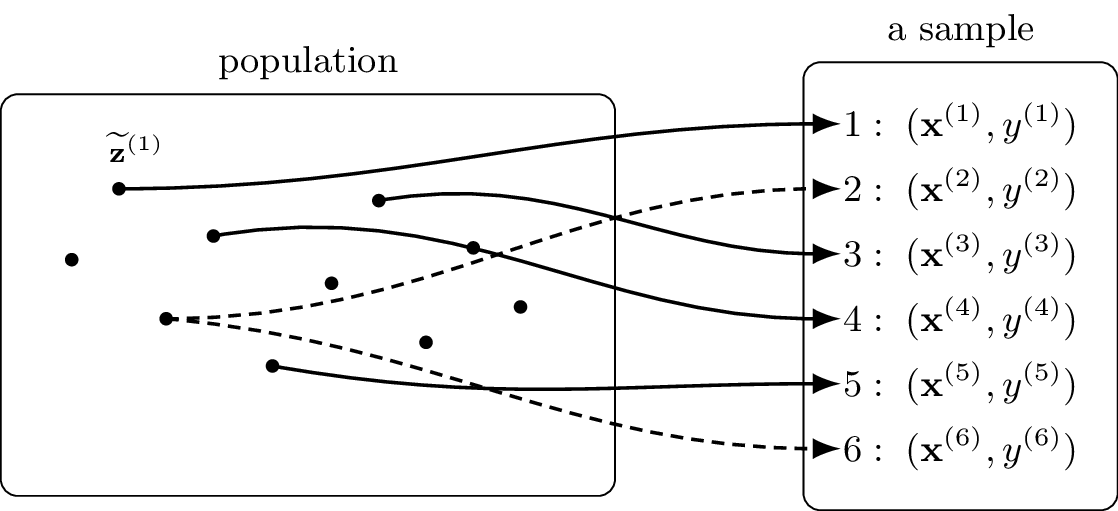
\includegraphics[width=0.8\linewidth]{../images/sample_tikz.png}
 \end{center}
 \caption{A sample viewed as a finite sequence.
 Each element of this sample consists of the feature vector
 and the label of a data point from an underlying population.
 The same data point may occur more than once in the sample.
 \label{fig:sample-sequence_dict}}
 \end{figure}
 For the analysis of machine learning (ML) methods, it is common to interpret (the generation of) a
 sample as the realization of a stochastic process indexed by $\{1,\ldots,m\}$.
 A widely used assumption is the independent and identically distributed assumption (i.i.d.\ assumption), where sample elements
 $\left( {\bf x}^{(r)},y^{(r)} \right)$,
 for $r=1,\ldots,m$, are independent and identically distributed (i.i.d.) random variables (RVs) with a common probability distribution. \\
 See also: dataset, sequence, independent and identically distributed assumption (i.i.d.\ assumption).

\end{document}
